\documentclass[]{article}
\usepackage[utf8]{inputenc}
\usepackage{amsmath}
\usepackage{pgfplots}
\usepackage{textcomp}
\pgfplotsset{width=10cm}
\pgfplotsset{holdot/.style={color=blue,fill=white,only marks,mark=*}}
%\usepgfplotslibrary{fillbetween}

\title{Noah's Guide to Calculus}
\author{Noah Stockwell}
\date{Summer 2016}

\begin{document}

\maketitle
\vspace{2in}
\begin{center}
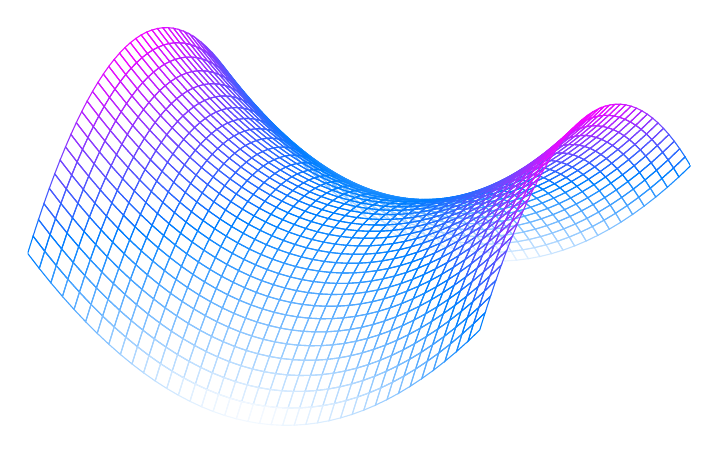
\begin{tikzpicture}
\begin{axis}[
hide axis,
xlabel=$x$,ylabel=$y$,
%mesh/interior colormap name=hot,
colormap/cool, 
]
\addplot3[domain=-3:3,mesh,samples=40]
{x^2-y^2};
\end{axis}
\end{tikzpicture}
\end{center}
\newpage
\tableofcontents
\newpage
\section{Understanding Limits}
\subsection{Introduction} Limits are a way of skirting the normal rules of math. Without the knowledge of limits, whenever a function divides by 0 or involves $\infty$ in any way, calculations become impossible. Limits take the rules of math a little less seriously and can be used to calculate what a value ``should be''. A simple example of where limits come in handy is when there is a ``hole'' in a graph:
\begin{center}
\begin{tikzpicture}
	\begin{axis}
	\addplot[domain=0:4,blue]{x+2};
	\addplot[holdot] coordinates{(2,4)};
	\end{axis}
\end{tikzpicture}
\end{center}
$$f(x)=\frac{x^2-4}{x-2}$$
Because $f(x)$ divides by 0 when $x=2$, there can be no answer here. However, we can tell that $f(2)$ should be 4 ignoring the division by zero. We can tell this because as $x$ becomes greater and nearer to 2 (approaching $x=2$ from the left), the value of $f(x)$ approaches 4. Similarly, when $x$ decreases and becomes nearer to $x=2$ (approaching $x=2$ from the right), the value of $f(x)$ approaches 4. Therefore, as both sides of $x=2$ become closer and closer, they converge upon a single point: $f(2)=4$.
\subsection{Limits} Limits can help us with the preceding problem. A limit returns the value of a function that it should be. \textit{We define the limit to be equal to the point both sides of a graph approaches.} A simple way to write this is $\lim\limits_{x\to c^{+}}f(x)$ to represent the limit as $x$ increases to the value $c$ and $\lim\limits_{x\to c^{-}}f(x)$ to represent the limit as $x$ decreases to the value $c$. In other words, $\lim\limits_{x\to c^{+}}f(x)$ is the value we approach moving to the right towards $c$ and $\lim\limits_{x\to c^{-}}f(x)$ is the value we approach moving to the left towards $c$. We define $$\lim\limits_{x\to c} f(x)= \lim\limits_{x\to c^{+}} f(x)=\lim\limits_{x\to c^{-}}f(x)$$ If the limits moving to the left and moving to the right are not equal, the statement above is false and we say that the limit does not exist. For example, the limit as $x$ approaches 2 in this graph doesn't exist:
\begin{center}
	\begin{tikzpicture}
	\begin{axis}
	[
	domain=-2:6, restrict y to domain=-4:4,
	]
	\addplot[domain=-2:6,red,samples=50]{1/(x-2)};
	\end{axis}
	\end{tikzpicture}
\end{center}
\subsection{Applications of Limits} Limits are very useful when needing to find a value that shouldn't necessarily exist. We can use limits to calculate holes in graphs from what we saw earlier, but we can also use them to approach unapproachable values like $\infty$. As we can only approach $\infty$ from one side, we write the limit as $\lim\limits_{x\to\infty} f(x)$ for positive $\infty$ and $\lim\limits_{x\to\ -\infty} f(x)$ for $-\infty$.
\subsection{Calculating limits} Unfortunately, there's no simple and easy way to calculate limits. The simplest way is just to ``plug in'' to the function but at some points like holes in the graph or $\infty$, we don't have that luxury. Instead, we can reduce or rewrite equations and also apply some general common sense. For example, $\lim\limits_{x\to\infty} \frac{1}{x}$ must be 0 because as $x$ gets larger, $\frac{1}{x}$ gets smaller to some point at which it must be 0. Using reduction and logic, we may progress on to more complex ideas involving limits.
\pagebreak
\section{Derivatives}

\end{document}
